\title{1. Rovnice a nerovnice s absolutní hodnotou a odmocninou mocninou}
\author{Jakub Sláma (Marek Fuchs)}
\date{24.4.2025}

\maketitle



\section{Rovnice a nerovnice s absolutní hodnotou a odmocninou mocninou}

\subsection{Absolutní hodnota}
\subsubsection{Absolutní hodnota reálného čísla} 
Absolutní hodnotu reálného čísla $a$, kde $a\in\mathbb{R}$ označujeme $|a|$ a platí pro ni:
\begin{equation}
|a|=\left\{
        \begin{matrix}         
            a, & \mbox{pokud }a \ge 0\\ 
            -a, &\mbox{pokud }a < 0
         \end{matrix}\right.
\end{equation}
\\
Pro kladnou hodnotu platí: $|1|= 1$, pro zápornou hodnotu platí: $|-1| = -(-1) = 1$

\subsubsection{Geometrický význam}
Absolutní hodnota nám vyjadřuje vzdálenost obrazu tohoto čísla od počátku
    \begin{figure}[H]
        \centering
        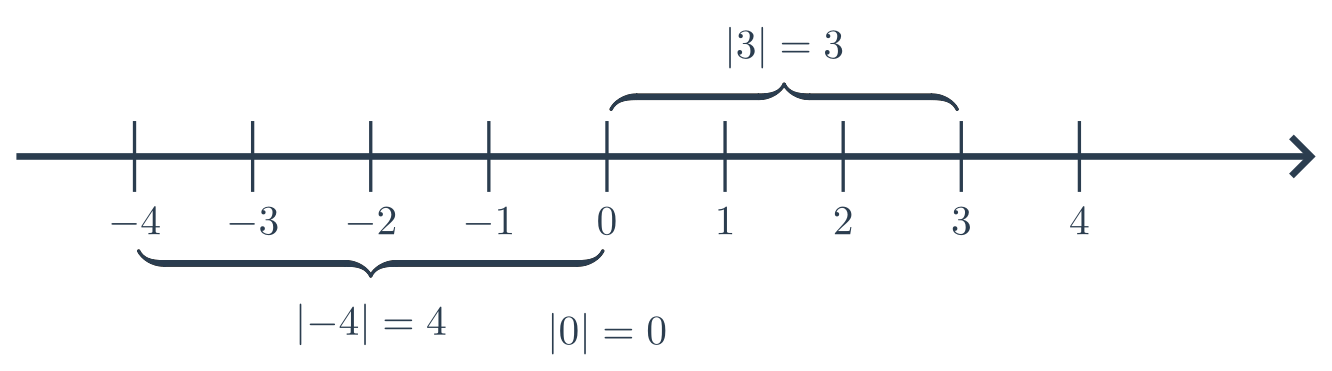
\includegraphics[width=0.5\linewidth]{img/ilustrace-absolutni-hodnota.png}
        \caption{Absolutní hodnota}
        \label{fig:enter-label}
    \end{figure}
\subsection{Mocnina a odmocnina z reálného čísla}
\textbf{Definice mocniny: }Pro libovolná reálná čísla $a$ a přirozená čísla $n$, kde:

\begin{itemize}
    \item $a$ je základ mocniny (říkáme mu základ nebo číslo, které umocňujeme)
    \item $n$ je exponent nebo mocnitel (říkáme mu stupeň nebo mocnina)
\end{itemize}
platí, že $a^n = a \cdot a \cdot a...$, tudíž: $a^3=a \cdot a \cdot a$
\subsubsection{Sudé mocniny, odmocniny}
Sudé mocniny jsou $a^x$, kde $x$ náleží celé sudé číslo např. $a^2; a^4; a^6$. Platí pro ně, že po umocnění čísla sudou mocninou bude výsledek vždy kladný.

Sudá odmocnina $\sqrt[x]{a}=n$, z nezáporného reálného čísla $a$ je takové nezáporné číslo $x$, pro které platí: $n^x = a; n\in\mathbb{R}^++\{0\}$.  Zapisujeme $\sqrt{a} = x$. Symbol $\sqrt{}$ se nazývá \textbf{odmocnítko}. Praxe: $\sqrt[2]{9}=3; \sqrt[2]{-9}=$ nelze v $\mathbb{R}$ (lze v $\mathbb{C}$).
\subsubsection{Liché mocniny, odmocniny}
Liché mocniny jsou $a^x$, kde $x$ náleží celé liché číslo např. $a^1; a^3; a^5$. Platí, že po umocnění čísla lichou mocninou bude výsledek se stejným znaménkem, jako základ.

Lichá odmocnina $\sqrt[x]{a}$, kde x náleží celému lichému číslu a $a \in\mathbb{R}$, platí: z reálného čísla \textbf{a} je reálné číslo \textbf{b}, pro které platí, že $b\cdot b \cdot b=a$ značíme $b=\sqrt[3]{a}$ Praxe: $\sqrt[3]{27}=3; \sqrt[3]{-27}=-3$. 


\subsubsection{Základní pravidla, pro počítání s mocninami a odmocninami}
Pro libovolné číslo $x \in \mathbb{R}$ a čísla $a,b,c,d \in \mathbb{Z}; b \land d\neq 0$ platí 
$$
    \sqrt[a]{x^b}=x^{\frac{b}{a}}, 
$$
$$
    x^\frac{a}{b} \cdot x^\frac{c}{d}=x^\frac{ad+cb}{bd}, \\
$$
$$
    (x^a)^b=x^{a \cdot b},
$$
$$
    \sqrt[a]{\sqrt[b]{x}} = \sqrt[a\cdot b]{x}.
$$
Přičemž číselný výsledek obecně $\in \mathbb{C}.$
\subsection{Ekvivalentní a důsledkové úpravy rovnic a nerovnic - rozdíly}
Při úpravách nerovnic používáme ekvivalentní úpravy, které se vyznačují tím, že nezmění platnost nerovnice. Smyslem ekvivalentních úprav je dostat nerovnici do jednoduššího tvaru. Výsledek rovnice s = je kořen/kořeny. Výsledek nerovnice je interval. Příklady rovnice a nerovnice:
$$
    3x+2=1+x
$$
$$
    |x+3| < 0
$$
\subsubsection{Ekvivalentní úpravy rovnic a nerovnic}
Ekvivalentní úpravy jsou takové, při kterých se nezmění počet výsledků rovnice, nebo nerovnice
\begin{itemize}
    \item přičtení výrazu 
    $$
        x-2=-2 /+2
    $$
    $$
        x-2+2=-2+2
    $$
    $$
        x=0
    $$
    \item odečtení výrazu
    $$
        x+2=2 /-2
    $$
    $$
        x+2-2=2-2
    $$
    $$
        x=0
    $$
    \item Vynásobení výrazem
    $$
        0,5x=3 / \cdot 2
    $$
    $$
        0,5x \cdot 2 = 3\cdot2
    $$
    $$
        x=6
    $$
    \item Vydělení výrazem
    $$
        3x=3 / \div3
    $$
    $$
        3x \div 3=3 \div 3
    $$
    $$
    x=1
    $$
    \end{itemize}
    Pokud násobíme nerovnici záporným číslem, potom musíme změnit znaménko nerovnosti.
    $$
        -x<1 / \cdot (-1)
    $$
    $$
        x>-1
    $$
\subsubsection{Důsledkové úpravy rovnic a nerovnic}
U důsledkových úprav (umocnění) získáme větší množství kořenů rovnice/nerovnice, tudíš musíme na konci výpočtu provést zkoužku (dosazení do původní rovnice/nerovnice a porovnání rovnosti pravé a levé strany), tímto způsobem vyřadíme nadbytečné nespávné výsledky.
\subsubsection{Rozdíly}

\begin{tabularx}{0.8\textwidth} { 
  | >{\raggedright\arraybackslash}X 
  | >{\centering\arraybackslash}X 
  | >{\raggedleft\arraybackslash}X | }
 \hline
 & Rovnice & Nerovnice\\
 \hline
 znaménko      &   $=$           & $\leq;<;>;\ge$\\
 násobení $-1$ &   nic se nemění & změna znaménka \\
 výsledek      &   n počet kořenů ($\mathbb{C}$) & interval \\
\hline
\end{tabularx}